\section{Introduction}
\subsection{Présentation du Shape-from-Shading}

Le Shape-from-Shading (SFS) est un problème fondamental en vision par ordinateur. Il consiste à reconstruire en 3D la surface d’un objet à partir des variations d’intensité lumineuse observées dans une image. Sous certaines hypothèses, ces variations permettent d’estimer les pentes de la surface, et donc de reconstruire la géométrie de l'objet. Lorsqu'on le formule d'un point de vue mathématique, on est amené à étudier une équation aux dérivées partielles (EDP) non linéaire d'ordre 1. Sa solution donne alors la hauteur ou la profondeur de l'objet étudié. 
Nous donnons ici un exemple de SFS appliqué à la reconstruction d'un vase artificiel. Cet exemple est issu de \cite{ref_vase}.

% insert 2 side by side redimensionned images
\begin{figure}[!htb]
    \begin{minipage}[t]{0.5\textwidth}
        \centering
        \fbox{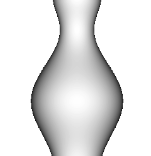
\includegraphics[width=.46\linewidth,height=4cm]{./Images/vase_tuto.png}}
        \caption{Intensité lumineuse d'un vase}\label{Fig:int_vase2}
    \end{minipage}\hfill
    \begin{minipage}[t]{0.5\textwidth}
        \centering
        \fbox{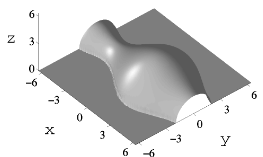
\includegraphics[width=.7\linewidth,height=4cm]{./Images/vase_tutor.png}}
        \caption{Vase reconstruit}\label{Fig:vase_tutor}
    \end{minipage}
\end{figure}

\subsection{Contexte historique}
Le problème du Shape-from-Shading est apparu dans les années 1970, à une époque où les chercheurs en vision par ordinateur commençaient à s’intéresser à la manière dont la lumière et l’ombre pouvaient être exploitées pour comprendre la géométrie des scènes. À cette époque, le SFS consistait principalement à reconstituer la forme d’objets à partir d’images en niveaux de gris. Cependant, avec le développement des technologies, plusieurs variantes du Shape-from-Shading ont été développées pour faire face à des situations plus complexes rencontrées dans des scènes réelles. On distingue par exemple 
\begin{itemize}
    \item Le \textbf{SFS classique}, avec une seule source lumineuse et un unique objet dans la scène. 
    \item Le \textbf{SFS à plusieurs lumières}, où l'objet est éclairé par plusieurs lumières. La multiplicité des sources de lumière permet d'obtenir plus d'informations sur l'objet. Cependant, la modélisation devient bien plus compliquée.
    \item Le \textbf{SFS à plusieurs objets}, qui s’intéresse à la reconstruction de scènes qui contiennent plusieurs objets qui peuvent en partie se chevaucher/superposer/cacher du point de vue de l'observateur.
    \item Le \textbf{SFS non lambertien}, qui tient compte des matériaux de l'objet. 
\end{itemize}

Ces différentes variantes démontrent la diversité des problèmes de SFS. De nos jours, l'utilisation du Shape-from-Shading est assez spécifique mais plutôt utile dans l'imagerie médicale et notamment dans la radiographie. Celui-ci intervient aussi dans l'inspection industrielle. En effet, le SFS est utilisé dans le contrôle qualité de pièces mécaniques (trouver des aspérités/irrégularités à la surface d'un objet). 
L’un des travaux fondateurs dans ce domaine est celui de B.K.P. Horn en 1975 \cite{Horn 1975}, qui a posé les bases mathématiques du problème en liant l’intensité lumineuse d’un pixel à l’orientation locale de la surface. Il voulait notamment appliquer le SFS à la représentation de la lune et à la vision par robot. Par \og vision par robot \fg{} nous entendons la capacité des machines à détecter et analyser des images ou des vidéos afin de prendre des décisions.


\subsection{Mise en équation du problème} 

Comme nous l'avons énoncé plus haut, le problème de SFS se réduit, sous les bonnes hypothèses, à résoudre une EDP non linéaire d'ordre 1. Nous souhaitons dans cette partie présenter les hypothèses de base afin de comprendre pourquoi une telle équation modélise correctement le problème. Cette modélisation est issue des travaux de Horn dans \cite{Horn 1986}.\\

Une \textbf{surface lambertienne} est une surface suivant la loi de Lambert. C'est-à-dire qu'elle ne produit pas de lumière spéculaire mais aussi que la quantité de lumière renvoyée est proportionnelle au cosinus de l’angle entre la lumière incidente et la normale à la surface. 

Un \textbf{angle solide} est une mesure de l'étendue d'un objet vu depuis un point donné. On le note $S$ et on l'exprime en stéradians (noté \(sr\)). Il est défini comme le rapport entre l'aire d'une portion de surface sphérique interceptée par un cône (ou toute forme tridimensionnelle) et le carré du rayon de la sphère: 
\begin{equation*}
    S=\frac{A \cos\left(\theta\right)}{r^2},
\end{equation*}
où $A$ représente l'aire de l'objet et $r$ la distance objet-observateur.

Par exemple, si on prend un disque de rayon 1m, situé à 1m de l'observateur, on aura $S={\pi} \ sr$. Si ce même disque se situe à 2m, on aura $S=\frac{\pi}{4}$ \(sr\). Il sera donc visuellement 4 fois plus petit. Enfin, si on incline le disque dans l'espace, visuellement on verra une ellipse et aura un angle solide plus faible.

\hspace{1.5cm}
\tdplotsetmaincoords{70}{110} % Adjust camera angles (theta, phi)
\begin{tikzpicture}[tdplot_main_coords, scale=3]
    % Base circle (cutting plane)
    \draw[thick] (0,0,0) circle (1);

    % Hemisphere (3D surface)
    \foreach \phi in {0,10,...,360} { % Longitude lines
        \draw[gray!50] 
            plot[domain=0:90, smooth, variable=\theta] 
            ({cos(\phi)*sin(\theta)}, {sin(\phi)*sin(\theta)}, {cos(\theta)});
    }
    \foreach \theta in {15,35,55,75} { % Latitude lines
        \draw[gray!50] 
            plot[domain=-180:180, smooth, variable=\phi] 
            ({cos(\phi)*sin(\theta)}, {sin(\phi)*sin(\theta)}, {cos(\theta)});
    }

    % --- Corrected curved rectangle patch ---
    \def\phiStart{-37}  % Longitude range
    \def\phiEnd{-22}
    \def\thetaStart{41} % Latitude range (from pole)
    \def\thetaEnd{53}

    % Calculate the four corners of the curved rectangle
    \coordinate (A) at ({cos(\phiStart)*sin(\thetaStart)}, {sin(\phiStart)*sin(\thetaStart)}, {cos(\thetaStart)});
    \coordinate (B) at ({cos(\phiEnd)*sin(\thetaStart)}, {sin(\phiEnd)*sin(\thetaStart)}, {cos(\thetaStart)});
    \coordinate (C) at ({cos(\phiEnd)*sin(\thetaEnd)}, {sin(\phiEnd)*sin(\thetaEnd)}, {cos(\thetaEnd)});
    \coordinate (D) at ({cos(\phiStart)*sin(\thetaEnd)}, {sin(\phiStart)*sin(\thetaEnd)}, {cos(\thetaEnd)});
    
    % Draw the curved patch
    \filldraw[red!20, draw=red, thick]
        plot[domain=\thetaStart:\thetaEnd, smooth, variable=\theta]
        ({cos(\phiStart)*sin(\theta)}, {sin(\phiStart)*sin(\theta)}, {cos(\theta)}) --
        plot[domain=\phiStart:\phiEnd, smooth, variable=\phi]
        ({cos(\phi)*sin(\thetaEnd)}, {sin(\phi)*sin(\thetaEnd)}, {cos(\thetaEnd)}) --
        plot[domain=\thetaEnd:\thetaStart, smooth, variable=\theta]
        ({cos(\phiEnd)*sin(\theta)}, {sin(\phiEnd)*sin(\theta)}, {cos(\theta)}) --
        plot[domain=\phiEnd:\phiStart, smooth, variable=\phi]
        ({cos(\phi)*sin(\thetaStart)}, {sin(\phi)*sin(\thetaStart)}, {cos(\thetaStart)}) --
        cycle;
    

    % Add red "S" label
    \node[red] at ({cos((\phiStart+\phiEnd)/2)*sin((\thetaStart+\thetaEnd)/2)}, 
    {sin((\phiStart+\phiEnd)/2)*sin((\thetaStart+\thetaEnd)/2)}, 
    {cos((\thetaStart+\thetaEnd)/2)}) {\large \(S\)};
    
    % --- Calculate projected rectangle corners ---
    \def\projectionDistance{1.5} % Distance for the projected rectangle
    
    % Project corner A
    \pgfmathsetmacro{\Ax}{cos(\phiStart)*sin(\thetaStart)}
    \pgfmathsetmacro{\Ay}{sin(\phiStart)*sin(\thetaStart)}
    \pgfmathsetmacro{\Az}{cos(\thetaStart)}
    \pgfmathsetmacro{\scale}{\projectionDistance/\Az}
    \coordinate (A') at ({\scale*\Ax}, {\scale*\Ay}, {\projectionDistance});
    
    % Project corner B
    \pgfmathsetmacro{\Bx}{cos(\phiEnd)*sin(\thetaStart)}
    \pgfmathsetmacro{\By}{sin(\phiEnd)*sin(\thetaStart)}
    \pgfmathsetmacro{\Bz}{cos(\thetaStart)}
    \pgfmathsetmacro{\scale}{\projectionDistance/\Bz}
    \coordinate (B') at ({\scale*\Bx}, {\scale*\By}, {\projectionDistance});
    
    % Project corner C
    \pgfmathsetmacro{\Cx}{cos(\phiEnd)*sin(\thetaEnd)}
    \pgfmathsetmacro{\Cy}{sin(\phiEnd)*sin(\thetaEnd)}
    \pgfmathsetmacro{\Cz}{cos(\thetaEnd)}
    \pgfmathsetmacro{\scale}{\projectionDistance/\Cz}
    \coordinate (C') at ({\scale*\Cx}, {\scale*\Cy}, {\projectionDistance});
    
    % Project corner D
    \pgfmathsetmacro{\Dx}{cos(\phiStart)*sin(\thetaEnd)}
    \pgfmathsetmacro{\Dy}{sin(\phiStart)*sin(\thetaEnd)}
    \pgfmathsetmacro{\Dz}{cos(\thetaEnd)}
    \pgfmathsetmacro{\scale}{\projectionDistance/\Dz}
    \coordinate (D') at ({\scale*\Dx}, {\scale*\Dy}, {\projectionDistance});
    
    % Draw the projected rectangle
    \filldraw[blue!20, draw=blue, thick] (A') -- (B') -- (C') -- (D') -- cycle;
    
    % Draw projection lines (dotted lines from origin through curved rectangle corners to projected rectangle corners)
    \draw[dashed, thick] (0,0,0) -- (A) -- (A');
    \draw[dashed, thick] (0,0,0) -- (B) -- (B');
    \draw[dashed, thick] (0,0,0) -- (C) -- (C');
    \draw[dashed, thick] (0,0,0) -- (D) -- (D');

    \pgfmathsetmacro{\midPhi}{(\phiStart+\phiEnd)/2}
    \pgfmathsetmacro{\midTheta}{(\thetaStart+\thetaEnd)/2}
    % Calculate projected center (P') and patch center (P)
    \coordinate (P) at ({cos(\midPhi)*sin(\midTheta)}, {sin(\midPhi)*sin(\midTheta)}, {cos(\midTheta)});
    \pgfmathsetmacro{\scale}{\projectionDistance/cos(\midTheta)}
    \coordinate (P') at ({\scale*cos(\midPhi)*sin(\midTheta)}, {\scale*sin(\midPhi)*sin(\midTheta)}, {\projectionDistance});
    
    % Draw blue projection line (r)
    \draw[<->, thick, blue] (0,0,0) -- (P') node[very near end, below] {\(r\)};
    
    % --- Calculate surface normal and incidence angle ---
    % For a flat rectangle in 3D, we need two edge vectors to calculate the normal
    % Edge vector 1: from A' to B'
    \pgfmathsetmacro{\edgeOneX}{\scale*\Bx - \scale*\Ax}
    \pgfmathsetmacro{\edgeOneY}{\scale*\By - \scale*\Ay}
    \pgfmathsetmacro{\edgeOneZ}{0} % Both points have same z-coordinate
    
    % Edge vector 2: from A' to D'
    \pgfmathsetmacro{\edgeTwoX}{\projectionDistance/\Dz*\Dx - \scale*\Ax}
    \pgfmathsetmacro{\edgeTwoY}{\projectionDistance/\Dz*\Dy - \scale*\Ay}
    \pgfmathsetmacro{\edgeTwoZ}{0} % Both points have same z-coordinate
    
    % Cross product to get normal vector (simplified since z-components are 0)
    \pgfmathsetmacro{\normalX}{0}
    \pgfmathsetmacro{\normalY}{0}
    \pgfmathsetmacro{\normalZ}{1} % The rectangle is in a plane parallel to xy-plane, so normal is (0,0,1)
    
    % Actually, let's use the correct normal for the projected rectangle
    % Since all points have the same z-coordinate, the normal is simply (0,0,1)
    
    % Center of the projected rectangle
    \pgfmathsetmacro{\centerX}{(\scale*\Ax + \scale*\Bx + \projectionDistance/\Cz*\Cx + \projectionDistance/\Dz*\Dx)/4}
    \pgfmathsetmacro{\centerY}{(\scale*\Ay + \scale*\By + \projectionDistance/\Cz*\Cy + \projectionDistance/\Dz*\Dy)/4}
    \pgfmathsetmacro{\centerZ}{\projectionDistance}
    
    % Vector from origin to rectangle center (incident ray direction)
    \pgfmathsetmacro{\incidentX}{\centerX}
    \pgfmathsetmacro{\incidentY}{\centerY}
    \pgfmathsetmacro{\incidentZ}{\centerZ}
    
    % Normalize the incident vector
    \pgfmathsetmacro{\incidentLength}{sqrt(\incidentX*\incidentX + \incidentY*\incidentY + \incidentZ*\incidentZ)}
    \pgfmathsetmacro{\incidentUnitX}{\incidentX/\incidentLength}
    \pgfmathsetmacro{\incidentUnitY}{\incidentY/\incidentLength}
    \pgfmathsetmacro{\incidentUnitZ}{\incidentZ/\incidentLength}
    
    % Length for drawing vectors
    \def\vectorLength{0.4}
    
    % Rectangle center coordinate
    \coordinate (RectCenter) at (\centerX, \centerY, \centerZ);
    
    % End point of normal vector (pointing outward from rectangle)
    \coordinate (NormalEnd) at ({\centerX}, {\centerY}, {\centerZ + \vectorLength});
    
    % End point of incident vector (pointing outward from rectangle center)
    \coordinate (IncidentEnd) at ({\centerX + \vectorLength*\incidentUnitX}, {\centerY + \vectorLength*\incidentUnitY}, {\centerZ + \vectorLength*\incidentUnitZ});
    
    % Draw the normal vector (green)
    \draw[->, thick, green!70!black] (RectCenter) -- (NormalEnd);% node[above] {\small normale};
    
    % Draw the incident ray direction (red, pointing outward from the surface)
    \draw[->, thick, red!70!black] (RectCenter) -- (IncidentEnd);% node[right] {\small incident};
    
    % Calculate angle between normal and incident ray
    % cos(θ) = normal · incident = (0,0,1) · (incidentUnitX, incidentUnitY, incidentUnitZ) = incidentUnitZ
    \pgfmathsetmacro{\cosTheta}{\incidentUnitZ}
    \pgfmathsetmacro{\thetaDegrees}{acos(\cosTheta)}
    
    % Draw angle arc
    % Parameters for arc
    \def\arcRadius{0.15}
    \pgfmathsetmacro{\arcSteps}{20}

    % Basis vector 1: normalized normal vector (already (0,0,1))
    \def\nx{0}
    \def\ny{0}
    \def\nz{1}

    % Basis vector 2: orthogonal component of incident vector (r) to the normal
    \pgfmathsetmacro{\rx}{\incidentUnitX}
    \pgfmathsetmacro{\ry}{\incidentUnitY}
    \pgfmathsetmacro{\rz}{\incidentUnitZ}

    % Compute projection of r onto plane orthogonal to normal (i.e., remove normal component)
    \pgfmathsetmacro{\dotProduct}{\nx*\rx + \ny*\ry + \nz*\rz}
    \pgfmathsetmacro{\vx}{\rx - \dotProduct*\nx}
    \pgfmathsetmacro{\vy}{\ry - \dotProduct*\ny}
    \pgfmathsetmacro{\vz}{\rz - \dotProduct*\nz}

    % Normalize v
    \pgfmathsetmacro{\vLength}{sqrt(\vx*\vx + \vy*\vy + \vz*\vz)}
    \pgfmathsetmacro{\vx}{\vx/\vLength}
    \pgfmathsetmacro{\vy}{\vy/\vLength}
    \pgfmathsetmacro{\vz}{\vz/\vLength}

    % Arc: sweep angle from 0 to thetaDegrees in the normal-incident plane
    \foreach \i in {0,...,\arcSteps} {
        \pgfmathsetmacro{\angle}{\i*\thetaDegrees/\arcSteps}
        \pgfmathsetmacro{\cosA}{cos(\angle)}
        \pgfmathsetmacro{\sinA}{sin(\angle)}
        
        % Point on arc: radius*(cos*normal + sin*v)
        \pgfmathsetmacro{\x}{\arcRadius*(\cosA*\nx + \sinA*\vx)}
        \pgfmathsetmacro{\y}{\arcRadius*(\cosA*\ny + \sinA*\vy)}
        \pgfmathsetmacro{\z}{\arcRadius*(\cosA*\nz + \sinA*\vz)}
        
        \coordinate (Arc\i) at ({\centerX+\x}, {\centerY+\y}, {\centerZ+\z});
    }

    % Draw arc as path
    \foreach \i [evaluate=\i as \next using int(\i+1)] in {0,...,\numexpr\arcSteps-1} {
        \draw[thick, orange] (Arc\i) -- (Arc\next);
    }

        
    % Label θ at midpoint of arc
    \pgfmathsetmacro{\midAngle}{\thetaDegrees/2}
    \pgfmathsetmacro{\cosMid}{cos(\midAngle)}
    \pgfmathsetmacro{\sinMid}{sin(\midAngle)}
    \pgfmathsetmacro{\lx}{\arcRadius*(\cosMid*\nx + \sinMid*\vx)}
    \pgfmathsetmacro{\ly}{\arcRadius*(\cosMid*\ny + \sinMid*\vy)}
    \pgfmathsetmacro{\lz}{\arcRadius*(\cosMid*\nz + \sinMid*\vz)}
    \node[above, orange] at ({\centerX+\lx}, {\centerY+\ly}, {\centerZ+\lz}) {\(\theta\)};

    
    % Add center point
    \node[scale=1.5, text=black] at (0,0,0) {\(\times\)};
    \node[below] at (0,0,0) {\(O\)};

\end{tikzpicture}

\vspace{-1cm} % Optional: reduce space between image and legend
\hspace{2cm}
\begin{tikzpicture}[remember picture, overlay]
    % 2D legend overlaid on the page, like a sticker
    \begin{scope}[shift={(8.5,2)}] % Position of the legend
        \draw[thick, fill=white] (0,-0.1) rectangle (4.7,3.3); % Adjusted height for spacing
        \node at (2.35,3) {\textbf{Légende}}; % Title

        % Vertical spacing unit (starting from top)
        \def\ybase{2.5}
        \def\ysep{0.4}

        % Red patch legend entry
        \fill[red!20, draw=red, thick] (0.2,\ybase) rectangle (0.5,\ybase+0.2);
        \node[right] at (0.6,\ybase+0.1) {Angle solide (\(S\))};

        % Blue patch legend entry
        \pgfmathsetmacro{\y}{\ybase - 1*\ysep}
        \fill[blue!20, draw=blue, thick] (0.2,\y) rectangle (0.5,\y+0.2);
        \node[right] at (0.6,\y+0.1) {Surface (\(A\))};

        % Dotted lines legend entry
        \pgfmathsetmacro{\y}{\ybase - 2*\ysep}
        \draw[dashed, thick] (0.2,\y+0.1) -- (0.5,\y+0.1);
        \node[right] at (0.6,\y+0.1) {Lignes de projection};

        % Blue vector legend entry
        \pgfmathsetmacro{\y}{\ybase - 3*\ysep}
        \draw[<->, thick, blue] (0.2,\y+0.1) -- (0.5,\y+0.1);
        \node[right] at (0.6,\y+0.1) {Distance (\(r\))};

        % Normal vector legend entry
        \pgfmathsetmacro{\y}{\ybase - 4*\ysep}
        \draw[->, thick, green!70!black] (0.2,\y+0.1) -- (0.5,\y+0.1);
        \node[right] at (0.6,\y+0.1) {Surface normale};

        % Incident vector legend entry
        \pgfmathsetmacro{\y}{\ybase - 5*\ysep}
        \draw[->, thick, red!70!black] (0.2,\y+0.1) -- (0.5,\y+0.1);
        \node[right] at (0.6,\y+0.1) {Rayon incident};

        % Angle arc legend entry
        \pgfmathsetmacro{\y}{\ybase - 6*\ysep}
        \draw[-, thick, orange] (0.2,\y+0.1) -- (0.5,\y+0.1);
        \node[right] at (0.6,\y+0.1) {Angle d'incidence (\(\theta\))};
    \end{scope}
\end{tikzpicture}
~\\



Nous cherchons à former une équation pour la carte de réflectance, c'est-à-dire une équation de la quantité de lumière renvoyée par la surface de l’objet en fonction de sa forme. Nous supposerons que cet objet possède une surface lambertienne. Pour ce faire, cherchons une relation entre la luminosité réfléchie par un élément de surface de l'objet et la luminosité perçue par cet élément de surface. \\

On pose $\delta O$ un élément de la surface à étudier (ex: $1mm^2$ du vase), $\delta \sigma$ un élément de la surface image (ex: image sur la photo du $mm^2$ de vase), $d$ le diamètre de la lentille formant l'image, $f$ sa focale (distance des centres lentille-images), $z$ la distance lentille-objet.
D'après les lois de l'optique géométrique, les angles solides de \(\delta O\) et $\delta \sigma$ vus depuis le centre de la lentille sont identiques: les rayons passant par le centre n'étant pas déviés. 

Ainsi, en posant $\alpha$ (respectivement $\theta$) l'angle entre la normale de $\delta \sigma$ (respectivement $\delta O$) avec le rayon incident, on a
\begin{equation*}
    \frac{\delta O \cos(\theta)}{(z/\cos(\alpha))^2}=\frac{\delta\sigma \cos(\alpha)}{(f/\cos(\alpha))^2}
\end{equation*}
Donc notamment 
\begin{equation*}
    \frac{\delta O}{\delta\sigma}=\frac{\cos(\alpha)z^2}{\cos(\theta)f^2}
\end{equation*}

La quantité de lumière que la surface $\delta\sigma$ reçoit est la même que la quantité de lumière que la lentille reçoit de la part de l'objet. Or l'angle solide de la lentille du point de vue de $\delta O$ est 
\begin{equation*}
    S=\frac{\pi \left(\frac{d}{2}\right)^2\cos(\alpha)}{(z/\cos(\alpha))^2}=\frac{\pi}{4}\left(\frac{d}{z}\right)^2\cos^3(\alpha)
\end{equation*}
Donc la puissance émise par $\delta O$ et reçue par la lentille, est 
\begin{equation*}
    \delta P= LS (\delta O\cos(\theta))
\end{equation*}
où $L$ représente l'éclairement énergétique de l'objet (on l'appelle aussi irradiance ou puissance lumineuse par unité de surface).\\
On peut définir la \textbf{radiance} comme \og la quantité de lumière reçue par une surface venant d'une direction spécifique \fg. Elle est exprimée en $W.m^{-2}.sr^{-1}$. L'\textbf{irradiance} est quand à elle \og la quantité totale de lumière reçue par une surface venant de toutes les directions\fg{} en $W.m^{-2}$.

On a alors 
\begin{equation*}
    E_i= \frac{\delta P}{\delta\sigma}=L\frac{\pi}{4}\left(\frac{d}{z}\right)^2\cos^4 \left( \alpha \right)
\end{equation*}
$E_i$ l'irradiance de notre surface image i.e sa luminosité. On remarque que $E_i$ est proportionnel à $L$ si on suppose $d,z,\alpha$ constants.\\

En général, l’irradiance reçue par une surface en fonction de la radiance de la lumière incidente dépend des angles d’incidence de la lumière (notés $(\theta_i,\phi_i)$) ainsi que des angles de vision de l’observateur. \\


Puisque nous considérons une surface lambertienne, on a par définition
L proportionnel à $\cos(\theta_i)$.\\

Regardons maintenant la surface à étudier sur l'ensemble $\Omega$. On note $u: \Omega \subset \R^2 \rightarrow \R$ la fonction définissant la hauteur de notre objet. Soit $\delta u$ la variation de hauteur de notre surface. En faisant un développement limité à l'ordre 1 nous obtenons 
\begin{equation*}
    \delta u(\delta x, \delta y)=\frac{\partial u}{\partial x}\delta x +o(\delta x)+ \frac{\partial u}{\partial y}\delta y +o(\delta y)
\end{equation*}
Ainsi la surface tangente à notre surface est engendrée par les vecteurs $(\delta x,0,\partial_xu \delta x)$ et $(0,\delta y, \partial_yu \delta y)$. En effectuant un changement de base on a 
\begin{equation*}
    \begin{split}
         r_x=(-1,0,-\partial_xu)\\
         r_y=(0,-1, -\partial_yu)
    \end{split}
\end{equation*}
La normale à cette surface est donc donnée par le produit vectoriel des deux vecteurs
\begin{equation*}
    n=\dfrac{r_x\wedge r_y}{|r_x\wedge r_y|}=\dfrac{(\partial_x u,\partial_yu, 1)}{\sqrt{1+(\partial_x u)^2+(\partial_y u)^2}}
\end{equation*}
Or nous avons L proportionnel à $\cos(\theta_i)$ avec $\cos(\theta_i)=n\cdot (\alpha,\beta,\gamma)$. Nous avons ici posé $(\alpha,\beta,\gamma)$ le vecteur normal d'incidence de la lumière (on peut le supposer constant si la source et l'observateur sont suffisamment éloignés de l'objet).\\

Nous normalisons alors l'irradiance de notre surface image  $E_i$ (proportionnel à $L$ donc à $\cos (\theta_i)$) et nous obtenons l'équation de la carte de réflectance 
\begin{equation*}
    R(n(x,y))=I(x,y)=n(x,y)\cdot(\alpha,\beta,\gamma)=\dfrac{\gamma+\alpha \partial_xu+\beta \partial_y u}{\sqrt{1+(\partial_xu)^2+(\partial_y u)^2}}
\end{equation*}
Cette équation peut se reformuler comme une équation d'Hamilton-Jacobi stationnaire d'ordre 1
\begin{equation*}
    I(x)\sqrt{1+|\nabla u|^2}-(\alpha,\beta)\cdot \nabla u-\gamma=0,\quad \forall x \in \Omega \subset \R^2.
\end{equation*}
Où l'Hamiltonien du problème est 
\begin{equation}\label{Hamiltonien}
    \boxed{H(x,p)=I(x)\sqrt{1+{\n{p}}^2}-(\alpha,\beta)\cdot p-\gamma, \quad x\in \Omega, \ p \in \R^2.}
\end{equation}
Le problème de Shape-from-Shading revient à résoudre l'équation $H(x,p)=0$ pour différentes fonctions $I$ qui dépendront des objets étudiés.


\subsection{Présentation du rapport}

Le papier \textit{A viscosity solutions approach to Shape-from-Shading} est un papier publié en 1992 par Élisabeth Rouy et Agnès Tourin \cite{Rouy_et_Turin}. Dans ce papier, les deux autrices reprennent les travaux de Horn et présentent une nouvelle méthode de résolution pour le problème de Shape-from-Shading. Elles proposent en effet de résoudre directement l'équation aux dérivées partielles $\eqref{Hamiltonien}$ avec une condition aux limites de Dirichlet $u=\varphi$ sur $\p\Omega$, en utilisant la théorie des solutions de viscosité développée par Lions et Crandall dans \cite{lion}. 

L'objectif du projet consiste à nous approprier le papier de Rouy et Tourin \cite{Rouy_et_Turin}. Par cela, nous entendons nous familiariser avec les notions de solutions de viscosité et les équations d'Hamilton-Jacobi. Nous avons aussi pour objectifs de comprendre et retrouver les différents résultats (théoriques et numériques) développés dans ce papier. Notre étude se concentre sur le Shape-from-Shading \og classique \fg.\\


Ce rapport est donc la synthèse de tous nos travaux réalisés pour ce projet. Dans la première partie, nous étudions d'un point de vue théorique l'Hamiltonien du problème. Nous commencerons par définir la notion de solution de viscosité. Nous donnerons ensuite deux résultats sur l'existence et l'unicité d'une solution pour l'équation $\eqref{Hamiltonien}$ qui est au centre de notre étude. Dans un second temps, nous mettrons en place un schéma numérique permettant d'approximer les solutions de viscosité de notre problème initial. Nous prouverons sa convergence et nous étudierons deux algorithmes d'approximation. La dernière partie est consacrée à la présentation de tous les résultats graphiques obtenus. Nous y présenterons la reconstruction d'un vase à la manière de celui de la \hyperref[Fig:vase_tutor]{Figure~\ref*{Fig:vase_tutor}} à l'aide de deux algorithmes, dont on comparera finalement l'efficacité.



